Oprogramowanie wszystkich elementów zostało napisane z~wykorzystaniem PlatformIO. Narzędzie pozwala na budowanie pod
systemy wbudowane na wiele platform \cite{pio-platforms}, w~tym wykorzystane do zbudowania sieci STMicroelectronics
STM32 Nucleo. Do kompilacji kodu źródłowego możliwe jest użycie wtyczki do edytora Visual Studio Code
\enquote{PlatformIO IDE} lub samodzielnego narzędzia CLI (ang. \textsl{Command Line Interface}) \enquote{PlatformIO
    Core}.

Rozwiązanie to zostało wybrane jako główne narzędzie do kompilacji oraz wgrywania kodu źródłowego, z~uwagi na to, że
działa na wielu plaformach. Dzięki temu nie jest wymagane instalowanie oraz ustawianie osobnych, dedykowanych środowisk
dla każdej z~wykorzystywanych platform. Jedynym wymogiem, aby móc zacząć pracę jest zainicjowanie projektu oraz
ustawienie podstawowej konfiguracji. Zadanie to jest bardzo proste, ponieważ dokumentacja narzędzia jest rozbudowana
i~bardzo szczegółowa.

\section{Rozpoczęcie projektu z~PlatformIO Core\label{sect:pio-intro}} Całość sieci składa się z~dwóch oddzielnych
projektów -- pierwszy z~nich to projekt uniwersalny dla modułów MASTER oraz SLAVE sieci LoRa, drugi natomiast
wykorzystywany jest do mikrokontrolera Adafruit Feather M0. Aby rozpocząć nowy projekt, należy wykorzystać komendę,
gdzie argumentem jest docelowy mikrokontroler:
\begin{verbatim}
   pio project init --board <board>
\end{verbatim}

W~przypadku projektu dla sieci LoRa wykorzystane zostały płytki Nucleo L152RE, stąd argumentem było
\texttt{nucleo\_l152}, natomiast dla projektu serwera sieci lokalnej -- \texttt{adafruit\_feather\_m0}. Użycie komendy
rozpoczyna proces tworzenia nowego projektu. Na podstawie podanego argumentu tworzony jest plik konfiguracyjny.
Zdefiniowane zostają platforma projektu oraz wykorzystywany framework. W~przypadku obu projektów wybrany został ten
wykorzystywany przez Arduino z~uwagi na dużą dostępność bibliotek, które działają bez potrzeby modyfikowania ich kodu
źródłowego. Dodatkowo zdefiniowana została tutaj prędkość transmisji portu szeregowego.

W~projekcie dla modułów sieci wykonana została modyfikacja pliku konfiguracyjnego -- elementy wygenerowane przez
narzędzie CLI PlatformIO przeniesione zostały do osobnej sekcji \texttt{[base\_config]}, natomiast konfiguracje dla
poszczególnych modułów znajdują się w~dedykowanych \enquote{środowiskach}. Wprowadzone zmiany zostały dokładniej opisane
w~sekcjach o~implementacji oprogramowania na poszczególne moduły (\ref{sect:firmware-network},
\ref{sect:firmware-webserver}).

Poza plikiem konfiguracyjnym, narzędzie generuje też podstawową strukturę plików całego. Powstaje folder \texttt{src},
który dedykowany jest dla plików źródłowych, \texttt{include} dla plików nagłówkowych, \texttt{lib} dla bibliotek
lokalnych oraz \texttt{tests} do testów jednostkowych, jeżeli planowane jest użycie ich.

\section{Praca z~PlatformIO\label{sect:pio-work}} Po stworzeniu projektu możliwe jest przystąpienie do pisania kodu
źródłowego na wybraną platformę. PlatformIO udostępnia możliwość kompilowania kodu oraz wgrywania go na docelowe
urządzenie poprzez jedną jedną komendę lub jeden przycisk w~edytorze tekstu. Jest to bardzo dobre rozwiązanie,
ponieważ dzięki temu możliwe jest skupienie się na rozwoju kodu źródłowego, zamiast czekania aż projekt będzie możliwy
do uruchomienia i~sprawdzenia.

\subsection{Uruchamianie projektu\label{sect:pio-run}} Uruchomienie projektu jest w~przypadku PlatformIO rozumiane
poprzez wykonanie kompilacji (\texttt{build}), wgranie skompilowanego kodu na urządzenie docelowe (\texttt{upload}) lub
wykonanie zdefiniowanego zestawu testów jednostkowych (\texttt{test}). Aby uruchomić projekt należy wykorzystać komendę:
\begin{verbatim}
   pio run [OPTIONS]
\end{verbatim}
Argumentami dodatkowymi mogą być:
\begin{itemize}[label=]
    \item \texttt{--environment}: element konfiguracji projektu, który określa zależności w~kwestiach
          kompilacji (np. flagi budowania projektu), programowania (wgrywania kodu) docelowych urządzeń, testów
          jednostkowych lub wykorzystanych bibliotek,
    \item \texttt{--target}: cel uruchomienia (np. kompilacja albo kombinacja kilku celów jednocześnie),
    \item \texttt{--upload-port}: port, do którego podłączone jest urządzenie i~na które ma zosatać wgrany kod.
          Szczególnie użyteczne w~przypadku, gdy pracuje się na wielu urządzeniach jednocześnie,
    \item \texttt{--monitor-port}: port, na którym po zakończeniu procesu ma zostać otwarty monitor portu szeregowego.
\end{itemize}
W~przypadku opcji związanych z~portem, jeżeli nie zostaną sprecyzowane (podane jako argument do komendy), PlatformIO
będzie próbował wykryć je automatycznie. Dostępne jest jeszcze kilka innych opcji, jednkże są one znacznie rzadziej
wykorzystywane, ponieważ ich domyślne opcje są tymi, które są najczęściej ustawiane.

\subsection{Zarządzanie bibliotekami\label{sect:pio-pkg}} PlatformIO posiada wbudowany moduł dedykowany do zarządzania
bibliotekami oraz innymi zasobami dołączanymi do projektu. Dzięki wykorzystaniu odpowiedniej podkomendy z~zestawu:
\begin{verbatim}
   pio pkg [COMMAND]
\end{verbatim}
możliwe jest przeszukiwanie, instalowanie z, aktualizacja lub publikowanie do rejestru dostępnych bibliotek. Podczas
wyszukiwania możliwe jest też zastosowanie filtrów, które w~znacznym stopniu zmniejszają ilość wyników i~przybliżają do
znalezienia tego pasującego. Wykorzysując tę operację zainstalowane zostały potrzebne do projektów biblioteki (wbudowane
dla frameworku Arduino, tak jak \enquote{Wire} czy te, które opublikowane zostały na platformie GitHub i~dodane do
rejestru PlatformIO). Na rys. \ref{img:pio-pkg-search} przedstawiony zostały przykładowy wynik wyszukiwania dostępnych
bibliotek związanych z~hasłem \enquote{LoRa}. Każdy wynik zawiera informację: nazwę, typ paczki, biblioteki, która
została znaleziona, najnowszą wersję, datę publikacji oraz krótki opis tego czym dana paczka, biblioteka są. Komenda
pokazuje także informacje o~tym ile wyników zostało znalezionych.

\begin{figure}[!htbp]
    \centering
    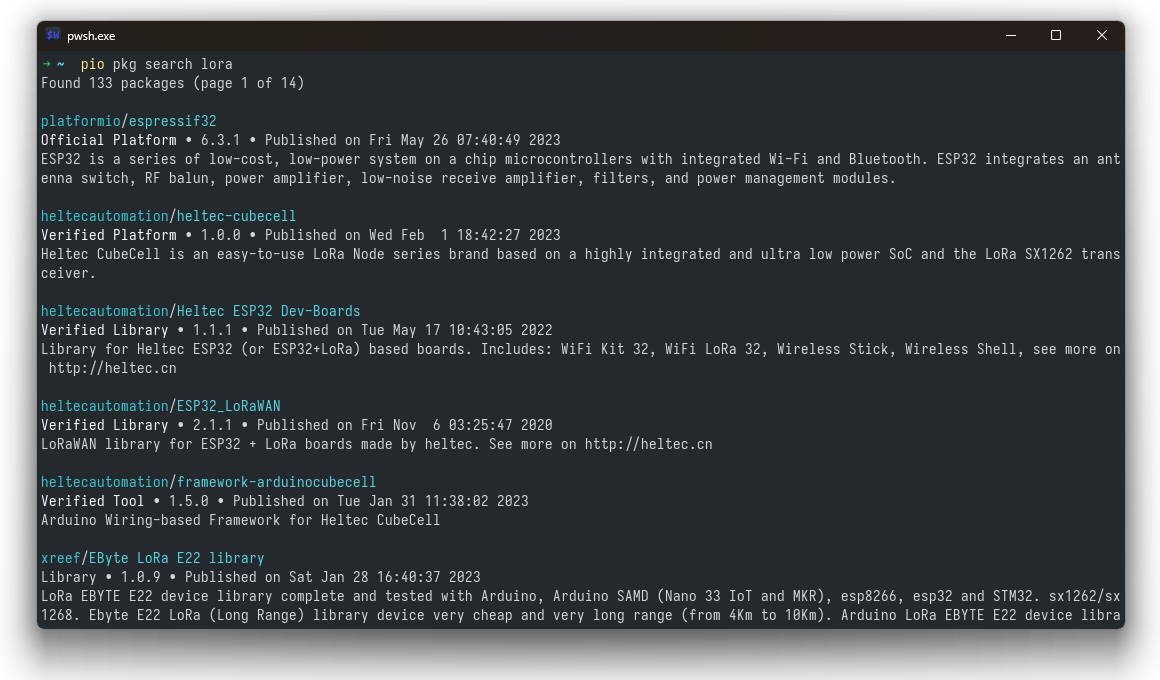
\includegraphics[width=1.0\textwidth]{screenshots/pio-pkg-search}
    \caption{\label{img:pio-pkg-search}Wyniki wyszukiwania bibliotek powiązanych z~hasłem \enquote{LoRa}}
\end{figure}